% -----------------------
% CHAPTER 2: LITERATURE REVIEW
% -----------------------
\chapter{LITERATURE SURVEY}
\label{ch:lit}
This chapter reviews three recent, highly relevant papers (2024--2025) focusing on modern phishing detection techniques, including machine learning, deep learning, graph neural networks, and blockchain integration. Each subsection presents a concise summary, the primary methods used, main advantages, and notable limitations.

\section{MLPhishChain: A Machine Learning-Based Blockchain Framework for Reducing Phishing Threats \cite{p1}}

This research presents \textbf{MLPhishChain}, a decentralized application (DApp) that mitigates the vulnerabilities of traditional centralized anti-phishing systems by integrating \textbf{machine learning (ML)} with \textbf{blockchain technology}. The proposed framework enables users to submit URLs for automated phishing analysis via a dedicated ML model (CheckPhish), with the resulting classification securely and permanently recorded on an immutable Ethereum-based ledger. 

Unlike conventional static blacklists that suffer from delayed detection and lack of transparency, MLPhishChain introduces a dynamic \textbf{re-evaluation mechanism}. This allows users to request updated assessments as website content evolves, ensuring the database remains accurate over time. Furthermore, the system integrates external security data from services like VirusTotal to provide a multi-source "second opinion," significantly enhancing the robustness of the URL verification process and boosting user confidence.

\newpage

% --- figure insertion ---
\begin{figure}[htbp]
  \centering
  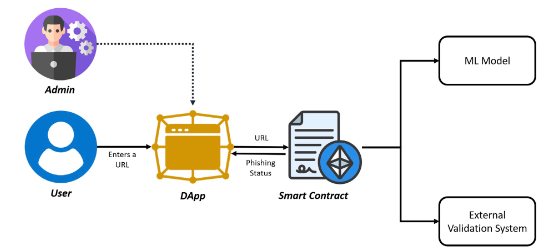
\includegraphics[width=1\textwidth]{assets/p1_diag.png}
  \captionsetup{justification=centering}
  \caption{The six components of the MLPhishChain architecture and their interactions}
  \label{fig:p1_diag}
\end{figure}

The figure illustrates the six primary components of the MLPhishChain framework and their operational workflow. The process centers around the \textbf{User}, who submits URLs through the \textbf{DApp} interface. The \textbf{Smart Contract} acts as the system's backbone, processing requests, querying the \textbf{ML Model} for initial phishing classification, and interacting with the \textbf{External Validation System} for secondary verification. It then records the confirmed statuses onto the blockchain. Finally, an \textbf{Admin} component is highlighted, representing the expert authority responsible for manually reviewing and resolving URLs that are flagged due to conflicting or changed classifications during the re-evaluation process.

\vspace{.5cm}

\textbf{Methods / Technology:} Ethereum smart contracts deployed via Ganache and Truffle; CheckPhish AI for core ML classification; VirusTotal API for external validation; Web3.js for DApp interaction.\\
\textbf{Advantages:} Eliminates centralized single points of failure; provides tamper-proof and transparent historical records; highly adaptable to evolving threats through its unique re-evaluation mechanism.\\
\textbf{Limitations:} Performance evaluations were conducted in a simulated environment (Ganache), which does not fully replicate real-world Ethereum Mainnet constraints such as high gas fees and network latency; currently relies on manual admin intervention to resolve re-evaluation discrepancies.\\

\vspace{-20pt}
\section{Phishing URL Detection Using Deep Learning: A Resilient Approach to Mitigating Emerging Cybersecurity Threats \cite{p2}}

This study proposes an advanced deep learning-based model designed to detect phishing URLs by processing raw text input, thereby eliminating the need for manual, domain-specific feature engineering. The framework integrates \textbf{character-level embeddings} with a hybrid \textbf{Parallel CNN-BiGRU architecture}. By combining Convolutional Neural Networks (CNNs) and Bidirectional Gated Recurrent Units (BiGRUs), the system is uniquely equipped to identify both localized obfuscation tactics and broader sequential anomalies in malicious links.

The model was trained and evaluated on a massive dataset of over 599,000 balanced URLs. The experimental results demonstrated exceptional performance, achieving a \textbf{98.46\% accuracy} rate and an AUC score of 99.62\%. The hybrid approach proved that parallel convolutional layers excel at extracting local features (like typo-squatting or suspicious substrings), while the BiGRU effectively captures the sequential relationships within the URL structure, resulting in a highly scalable and resilient detection mechanism.

% --- figure insertion ---
\begin{figure}[htbp]
  \centering
  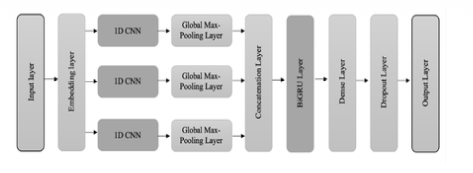
\includegraphics[width=.9\textwidth]{assets/p2_diag.png}
  \caption{Architecture of the proposed hybrid Parallel CNN-BiGRU deep learning model}
  \label{fig:p2_diag}
\end{figure}
\newpage

The figure illustrates the internal architecture of the proposed deep learning model. The process begins at the input layer, where raw URLs undergo tokenization and are passed through a \textbf{Character Embedding Layer} to transform them into dense numerical vectors. These vectors are then fed simultaneously into three \textbf{Parallel 1D CNN Layers} utilizing varying kernel sizes (3, 5, and 7). This parallel structure allows the network to capture multi-scale local spatial patterns, ranging from short deceptive prefixes to longer high-level structural anomalies.

Following global max-pooling, the outputs from the CNNs are concatenated and passed into a \textbf{BiGRU (Bidirectional Gated Recurrent Unit) Layer}. This layer processes the data in both forward and backward directions to capture long-range contextual dependencies within the URL string. Finally, the features are refined through a dense fully connected layer and a dropout layer (to prevent overfitting) before reaching the output layer, which uses a sigmoid activation function to generate the final probability score for classification.

\vspace{.5cm}

\textbf{Methods / Technology:} Character-level embedding; Parallel 1D CNNs (kernels 3, 5, 7); BiGRU for sequence modeling; SMOTE (Synthetic Minority Oversampling Technique) to handle dataset class imbalance.\\
\textbf{Advantages:} Completely bypasses manual feature engineering; highly accurate and balanced metrics (Precision/Recall $\sim$98.4\%); lightweight and computationally efficient (1.31 MB model size).\\
\textbf{Limitations:} The hybrid nature of utilizing multiple CNNs alongside BiGRU processing introduces higher computational overhead and longer training times compared to simpler standalone models; still susceptible to a small margin of false negatives (709 missed phishing URLs in testing).\\


\bigskip

\section{Phishing URL Detection using Graph Neural Networks and Rule-Based Models with Blockchain Integration \cite{p3}}

This paper proposes a highly robust hybrid phishing detection framework that tackles the accuracy-interpretability trade-off by combining \textbf{Graph Neural Networks (GNN)} with a \textbf{Rule-Based Model}, all backed by \textbf{blockchain integration}. While machine learning models offer strong detection rates, they often act as "black boxes." This system solves that by using the GNN to identify complex, hidden structural and relational properties between domains and URLs, while the Rule-Based Model applies transparent, heuristic rules (e.g., unusual domain lengths, suspicious keywords) to ensure the system's decisions are explainable.

The core of the framework is its \textbf{fusion logic}, which intelligently merges the confidence scores of the GNN with the heuristic explanations of the Rule-Based Model. If the models disagree, the logic weighs the outcomes and flags uncertainties. To guarantee the integrity of the system, the final verdicts, model confidence scores, and rule-based explanations are permanently logged onto a blockchain ledger, generating an immutable, tamper-free audit trail for cybersecurity analysts.

% --- figure insertion ---
\begin{figure}[htbp]
  \centering
  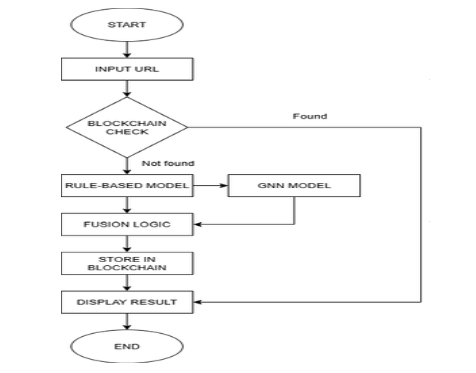
\includegraphics[width=1\textwidth]{assets/p3_diag.png}
  \caption{Operational workflow of the hybrid GNN and Rule-Based phishing detection system}
  \label{fig:p3_diag}
\end{figure}

\newpage

The figure outlines the step-by-step architectural workflow of the proposed detection system. When a user inputs a URL, the system first performs a \textbf{Blockchain Check} to determine if the URL has already been evaluated and recorded. If a match is found, the system immediately displays the immutable result, saving computational resources. 

If the URL is not found on the ledger, it is simultaneously processed by the \textbf{Rule-Based Model} and the \textbf{GNN Model}. The Rule-Based Model evaluates the link against established heuristics, while the GNN assesses its structural and relational graph properties. The outputs from both models are then fed into the \textbf{Fusion Logic} module, which resolves any discrepancies and synthesizes a final verdict. Once the decision is finalized, it is stored in the blockchain for future reference before the result is displayed to the end-user.

\vspace{.5cm}

\textbf{Methods / Technology:} Graph Neural Networks (GNN) for relational data analysis; Heuristic Rule-Based logic for explainability; Fusion mechanism for decision weighting; Blockchain ledger for immutable storage.\\
\textbf{Advantages:} Achieves an optimal balance between the high recall/pattern recognition of GNNs and the high precision/interpretability of rule-based systems; ensures absolute data integrity and auditability via decentralized logging.\\
\textbf{Limitations:} The standalone GNN module is prone to higher false positives (lower precision), while the rule-based model suffers from higher false negatives (lower recall); integrating these dual models alongside a blockchain write-mechanism significantly increases the overall architectural and computational complexity.

% -----------------------
% End of Chapter 2
% -----------------------